\documentclass[12pt,a4paper]{article}
\usepackage[spanish,es-tabla]{babel}
\usepackage{bbm}
\usepackage[utf8]{inputenc}
\usepackage{multicol}
\usepackage[T1]{fontenc}
\usepackage{graphicx}
\usepackage{gensymb}
\usepackage{amssymb, amsmath} %Paquetes matemáticos de la American Mathematical Society
\parskip=1 mm
\oddsidemargin -0.8 cm
\headsep -2 cm
\textwidth=17.8cm
\textheight=25.5cm
\begin{document}
\title{Laboratorio de Mecanica, Practica 3 - Densidad de un liquido}
\date{10 de febrero del 2025}
\author{\textbf{Ortega Montero Fernando Naed} - Equipo 4\\
Yibran Morales Munguía\\
Victor Manuel Santillan Romero}
\maketitle
\section{Resumen} 

En este reporte de laboratorio se realizo un ejercicio que consistió en la medición del volumen y masa de un liquido con ayuda de una balanza graduada con brazo y un vaso de precipitado, con el objetivo de obtener una grafica de puntos con la cual aproximar un modelo que describa de manera continua el volumen con relación a la masa.

\section{Introducción}

El objetivo de la practica fue medir la masa de un líquido (Con una balanza graduada con brazo) con relación a el volumen (con una Probeta), esto con el objetivo de plasmar los puntos en una recta y obtener la ecuación de una recta aproximada a estos puntos que sirva como modelo de los datos experimentales.\\
Para esto podemos ver que la ecuación de una recta es de la forma…
\[y = mx+ b\]
Donde $y$ será la masa, $x$ el volumen, $b$ será la masa de la probeta, y $m$ será la densidad.


\section{Desarrollo experimental}

Para la práctica se usó, un Vaso de precipitado, una balanza graduada con brazo con resolución de 0.1 g, una probeta con una resolución de 0.1 ml, una pipeta con una resolución de 1 ml, y un líquido. \\
Se midió a partir de los 2.5 ml con incrementos de 2.5 ml, se midió la masa de la probeta y a partir de ese punto se midieron 10 incrementos. \\

El líquido fue vertido en el vaso de precipitado y con ayuda de la pipeta se fue vertiendo el líquido y usando la balanza graduada con brazo se midió la masa.

\section{Resultados}

En la tabla podemos ver los resultados de las 10 mediciones, y la medicion 0 osea la medición de la probeta. y en la Figura 1 se puede ver ya la aproximación de la recta.\\


\begin{table}[h]
\begin{center}
\begin{tabular}{|c|c|c|}
\hline
& Volumen & Masa\\\hline
$M_0$ & 0 ml & 11.7 g\\\hline
$M_1$ & 2.5 ml & 13.9 g\\\hline
$M_2$ & 5.0 ml & 16.3 g\\\hline
$M_3$ & 7.5 ml & 19.0 g\\\hline
$M_4$ & 10.0 ml & 12.7 g\\\hline
$M_5$ & 12.5 ml & 24.2 g\\\hline
$M_6$ & 15.0 ml & 26.6 g\\\hline
$M_7$ & 17.5 ml & 29.2 g\\\hline
$M_8$ & 20.0 ml & 31.7 g\\\hline
$M_9$ & 22.5 ml & 34.2 g\\\hline
$M_10$ & 25.0 ml & 36.9 g\\
\hline
\end{tabular}
\end{center}
\end{table}

\begin{figure}[h!]
\centering
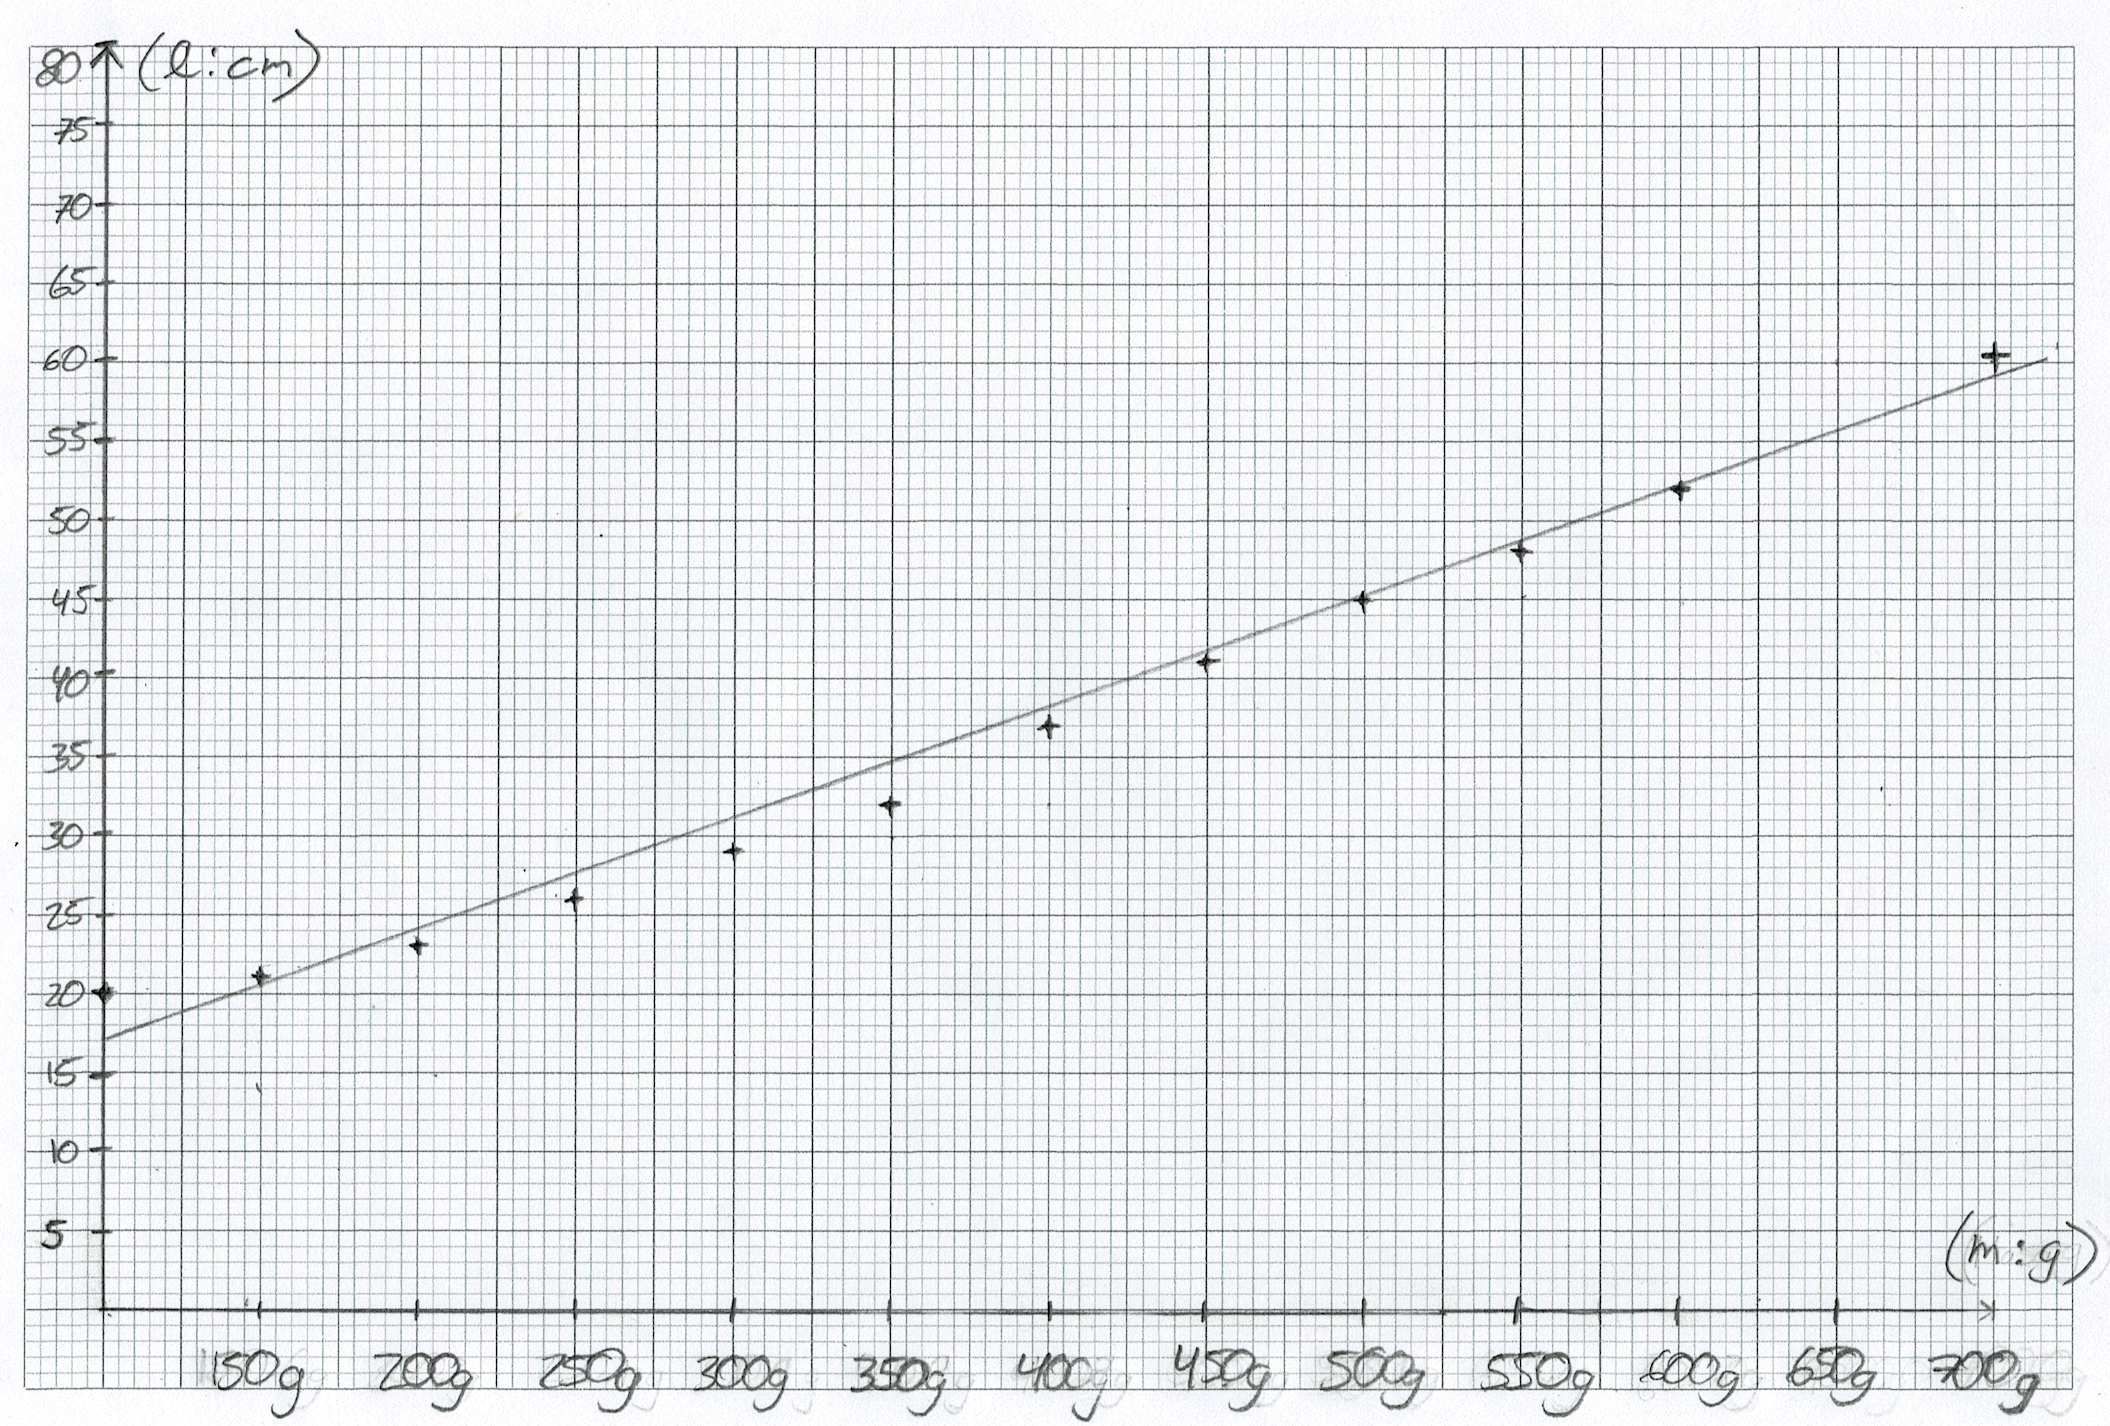
\includegraphics[scale=1]{1.jpg}
\caption{}
\end{figure}

\section{Discusión}

A pesar de no conocer realmente la composición del líquido o su densidad real, la práctica se llevó a cabo sin ninguna dificultad. 

\section{Conclusión}

La aproximación de la ecuación de una recta que describa un modelo ideal de la relación entre masa y volumen para obtener así la densidad de el liquido es una buena herramienta que puede a ayudar a hacer predicciones cuando no se pueda medir de manera correcta alguna de las variables ya descritas.  

\section{Referencias}

Martín, J. M. (2025) \textit{Física Experimental. Introducción a los conceptos y métodos.} Recuperado el 11, 02, 2025, de https://copitarxives.fisica.unam.mx/LT0006ES/LT0006ES.pdf 


\end{document}
